%!TEX root=../../main.tex
\section{Frontend}
In diesem Kapitel wird die Erstellung eines Konzepts für das Frontend erläutert. Dabei müssen Faktoren wie beispielsweise unsere Zielgruppe, die Lehrerschaft beachtet werden. Im folgenden Kapitel werden die theoretischen Hintergründe des Konzeptes überlegt, danach werden erste Entwürfe mittels Mockups erstellt. 
\subsection{Theoretische Konzeption}
Da die Zielgruppe \enquote{Lehrer} nicht gleichaltrig ist, sondern die darin enthaltenen Menschen ein Alter von 25 bis 65 Jahren haben gibt es keine Literatur zur \enquote{perfekten Usability für Lehrpersonal}. Daher richten wir uns nach dem Buch \enquote{Don't Make Me Think: A Common Sense Approche to Web Usability} von Steve Krug und an dem Buch \enquote{101 UX Principles} von Will Grant. Um eine gute Usability für die Lehrer des TGMs zu gewährleisten werden wir den Prozess der Entwicklung streng in Kontakt zu Lehrern begleiten und das Produkt auch mit nicht Technik affinen Menschen testen.  
\newpage
\subsection{Visuelle Konzeption}
\paragraph{Login-Seite}
~\\
Wie man auf der Abbildung 6.1 sehen kann ist die Login-Seite sehr schlicht gehalten. Neben dem Schriftzug \enquote{Refundable} soll das Formular zum einloggen sein. Da die Plattform nur für das Personal des TGMs zugänglich sein soll, wird bei der Eingabe der E-Mail Adresse automatisch eine \enquote{@tgm.ac.at} Adresse gefordert. Wird der \enquote{Passwort vergessen?} Link betätigt, soll automatisch auf die Seite des TGMs verwiesen werden, da wir über LDAP die Daten der Lehrer abrufen. Bei der Eingabe von validen Daten und des betätigen des \enquote{Anmelden} Buttons wird der Benutzer auf die Startseite weitergeleitet.
\begin{figure}[H]
	\centering
	
\includegraphics[width=1\linewidth]{images/Mockup-Startseite}
	\caption[Mockup Login]{Das Mockup der Login Seite}
	\label{fig:mockupLogin}
\end{figure}
Zur Veranschaulichung der oben genannten Prozesse ist in Abbildung 6.2 ein beispielhaftes Use-Case Diagramm zu sehen: 
\begin{figure}[H]
	\centering
	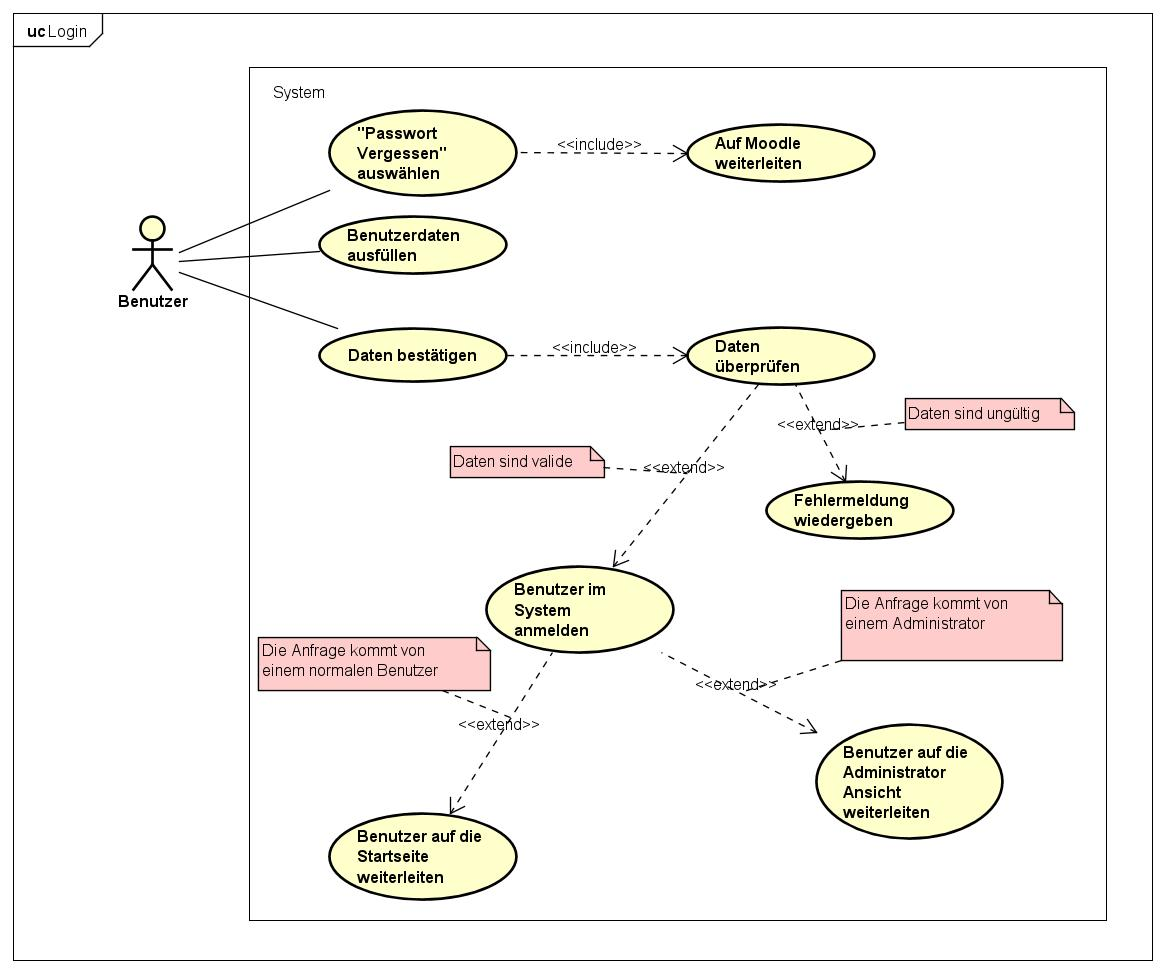
\includegraphics[width=1\linewidth]{images/uc-login}
	\caption[Use Case Diagramm Login]{Das Use Case Diagramm der Login Seite}
	\label{fig:ucLogin}
\end{figure}
\newpage
\paragraph{Startseite}
~\\
Die Startseite soll möglichst einfach gestaltet sein, damit selbst Lehrer, die keinen Bezug zur Technik haben sich auf den ersten Blick auskennen. Links auf der Abbildung 6.4 kann man entweder einen neuen Antrag erstellen, sich alle Anträge anzeigen lassen oder nur alle aktiven Anträge anzeigen lassen. Auf der rechten Seite soll man Neuigkeiten zu seinen aktiven Anträgen sehen können.
\begin{figure}[H]
	\centering
	
\includegraphics[width=1\linewidth]{images/Mockup-Startseite-eingeloggt}
	\caption[Mockup Startseite]{Das Mockup der Startseite, nachdem man sich eingeloggt hat}
	\label{fig:mockupStart}
\end{figure}
Zur Veranschaulichung der oben genannten Prozesse ist in Abbildung 6.4 ein beispielhaftes Use-Case Diagramm zu sehen: 
\begin{figure}[H]
	\centering
	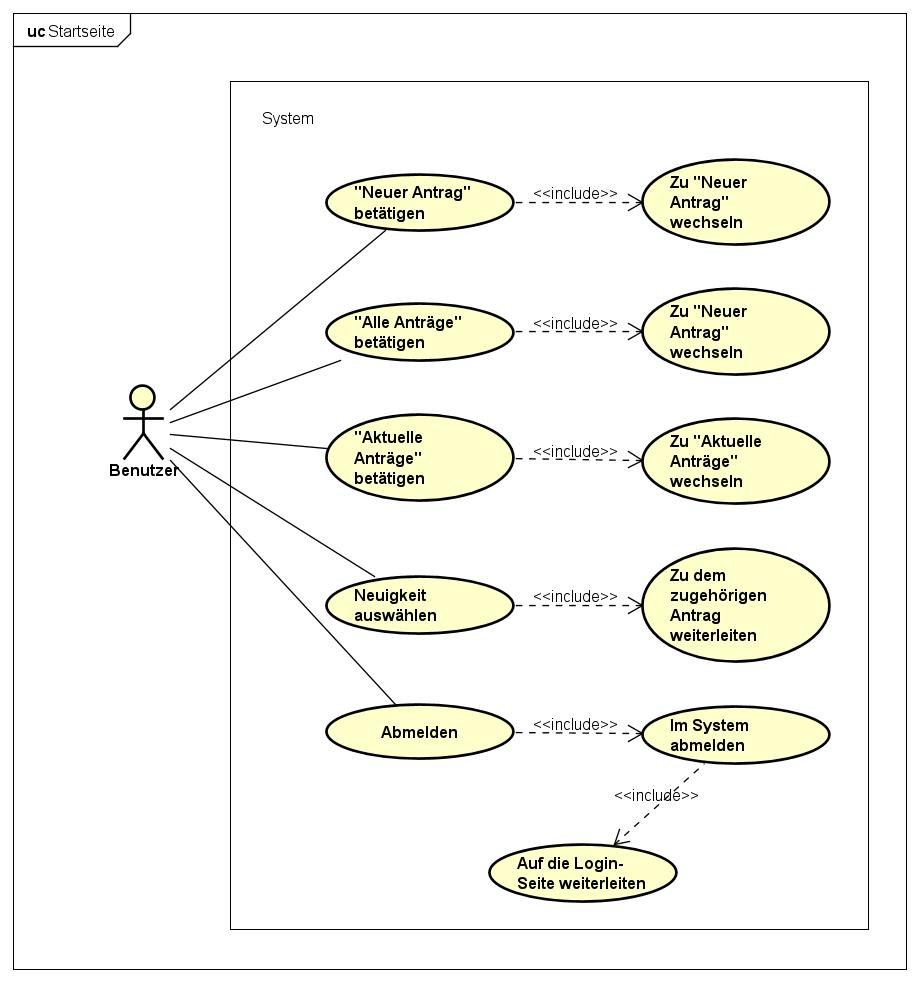
\includegraphics[width=1\linewidth]{images/uc-start}
	\caption[Use Case Diagramm Login]{Das Use Case Diagramm der Startseite}
	\label{fig:ucStart}
\end{figure}
\paragraph{Neuer Antrag}
~\\
Nachdem man auf den Button zum erstellen eines neues Antrages gedrückt hat, soll man zu einer Auswahl kommen, was für einen Antrag man erstellen möchte (Abbildung 6.5). Danach sollen je nach Antragsart, wie man auf der Abbildung 6.6 sieht Eingabefelder erscheinen, in denen die benötigten Daten zu dem Antrag eingetragen werden.
\begin{figure}[H]
	\centering
	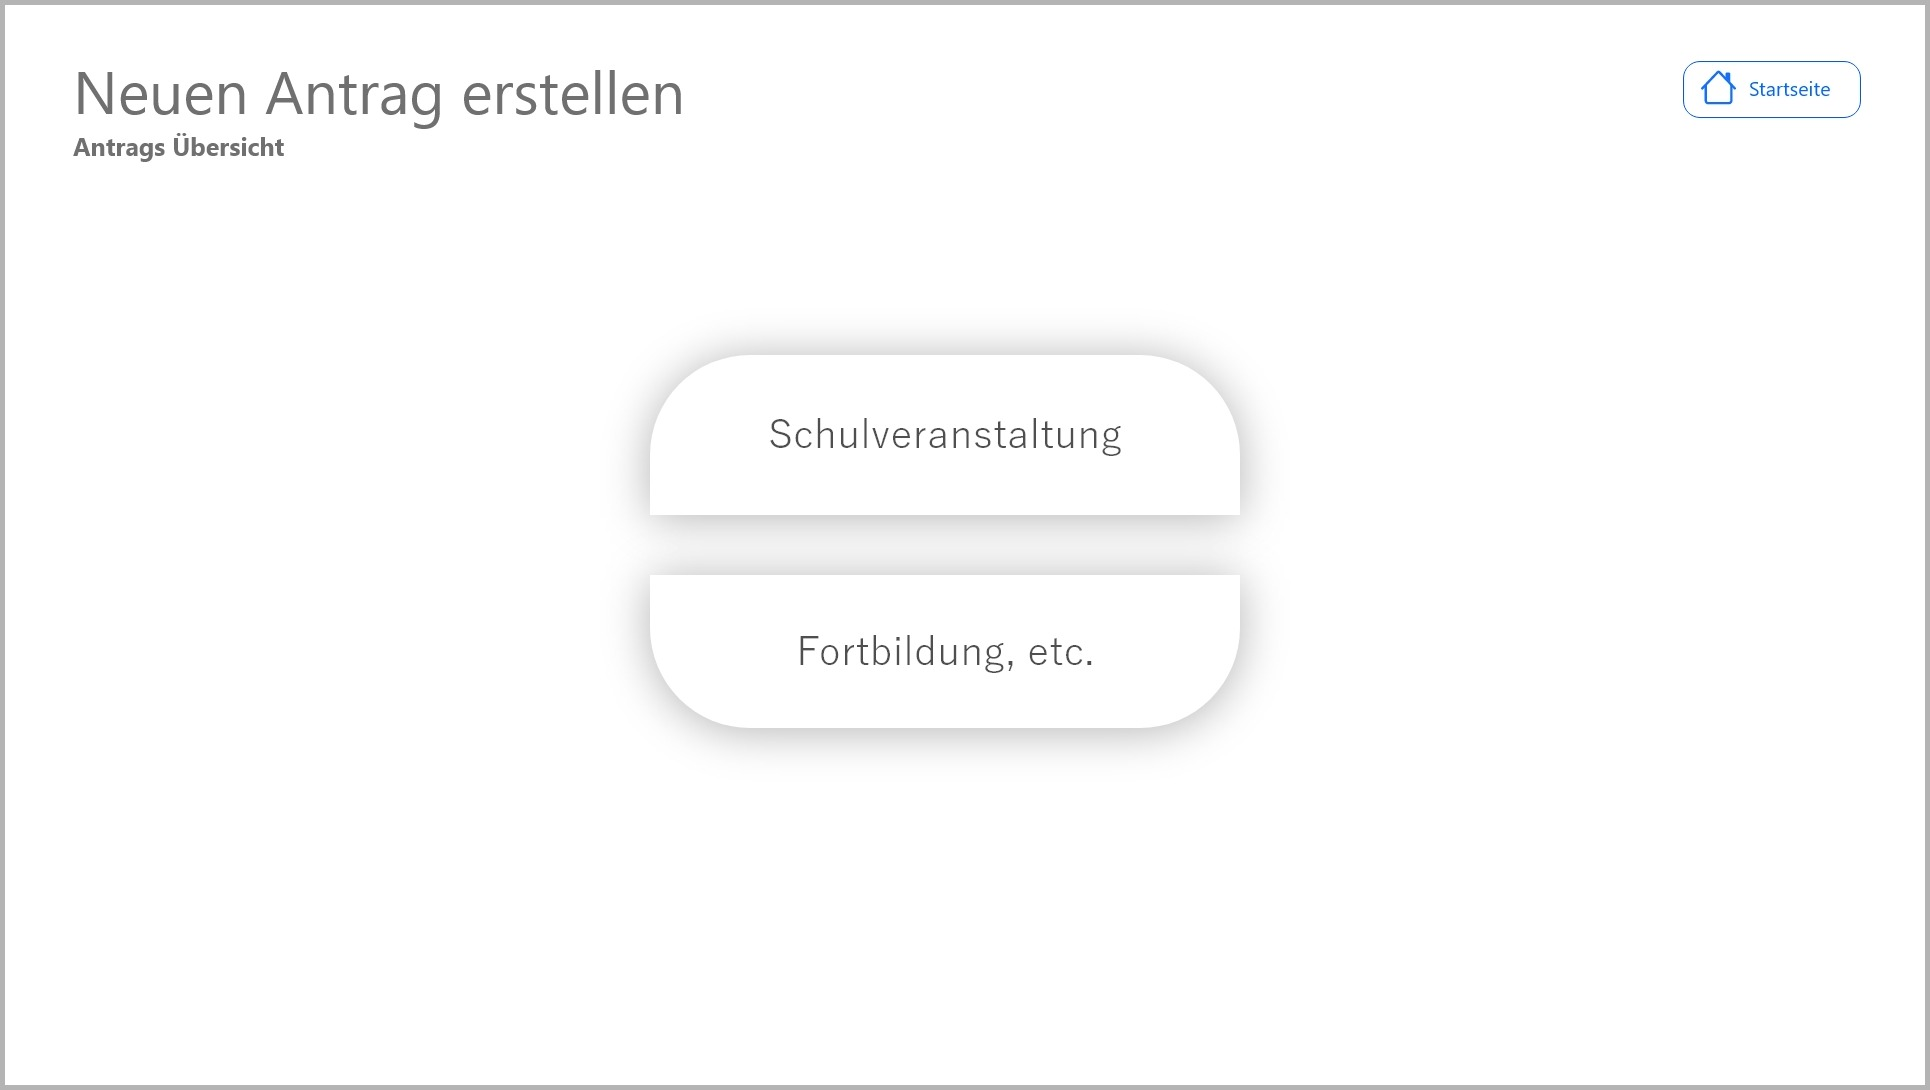
\includegraphics[width=1\linewidth]{images/Mockup-Neuer-Antrag}
	\caption[Mockup neuer Antrag]{Das Mockup der Seite, auf der man eine Antragsart auswählen kann}
	\label{fig:mockupNeu}
\end{figure}
\begin{figure}[H]
	\centering
	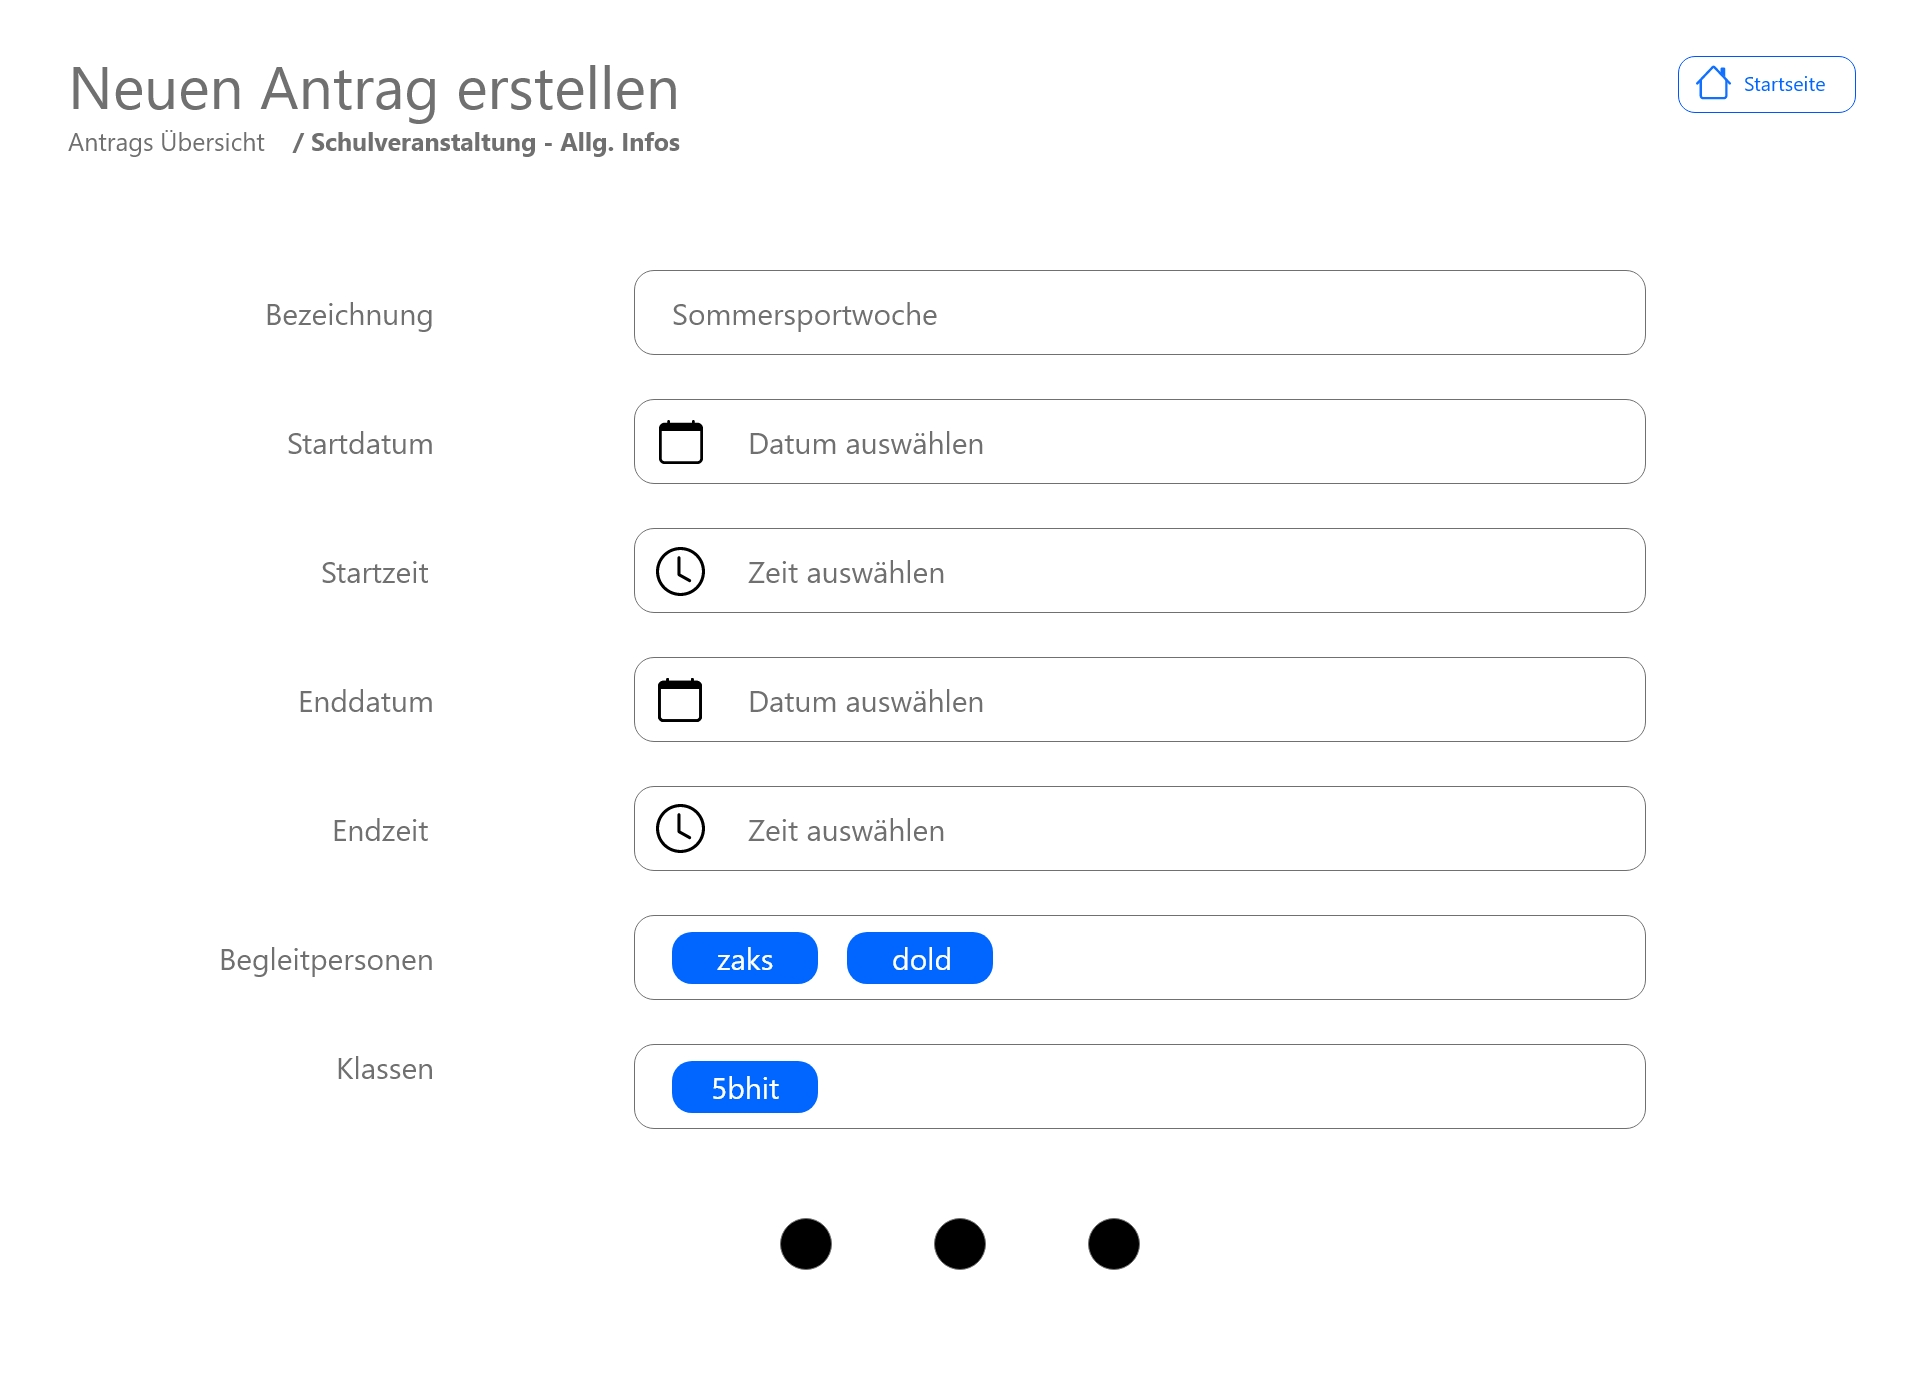
\includegraphics[width=1\linewidth]{images/Mockup-Antrag-erstellen}
	\caption[Mockup Antrag erstellen]{Das Mockup zum erstellen einer neuen Schulveranstaltung}
	\label{fig:mockupErstellen}
\end{figure}
Zur Veranschaulichung der oben genannten Prozesse ist in Abbildung 6.7 ein beispielhaftes Use-Case Diagramm zu sehen: 
\begin{figure}[H]
	\centering
	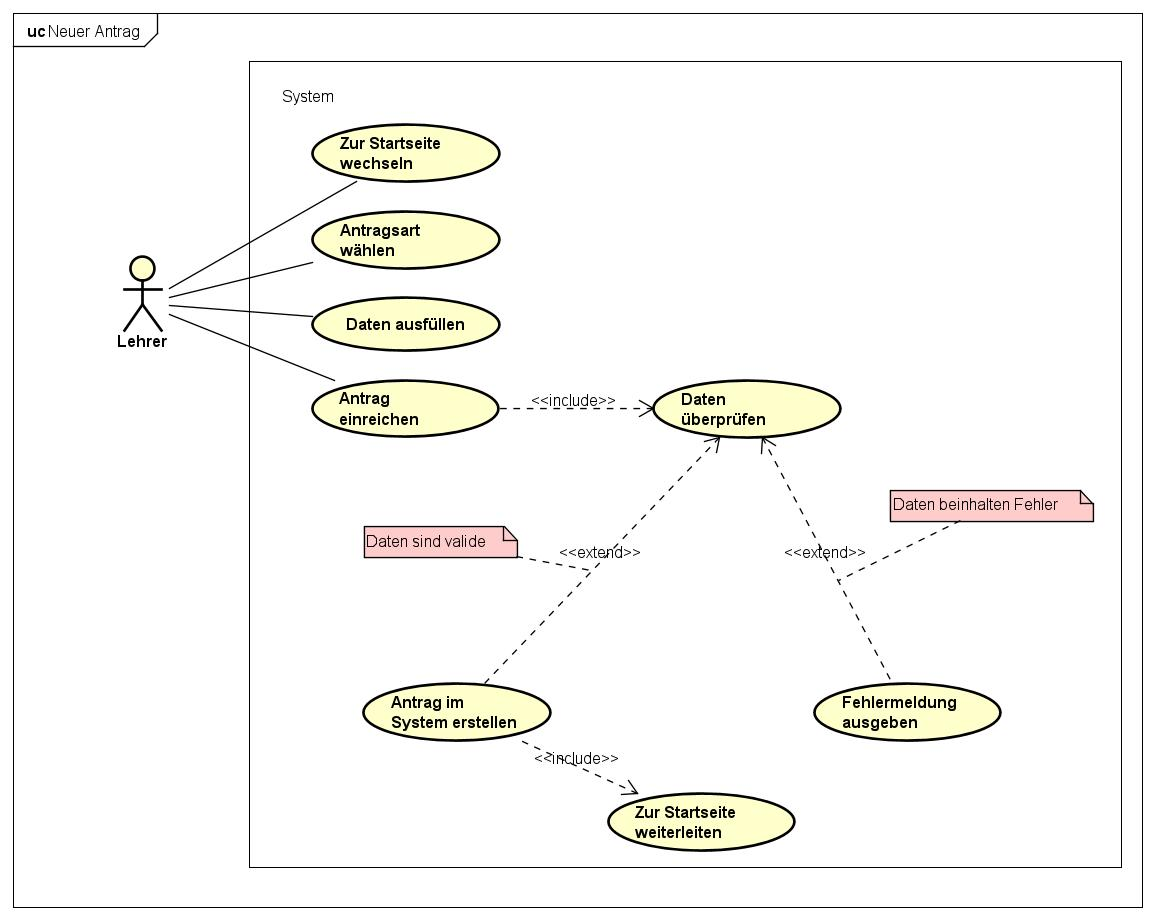
\includegraphics[width=1\linewidth]{images/uc-new}
	\caption[Use Case Diagramm Neuer Antrag]{Das Use Case Diagramm vom erstellen eines neuen Antrages}
	\label{fig:ucStart}
\end{figure}
\newpage
\paragraph{Ansicht Alle Anträge}
~\\
Auf der \enquote{Alle Anträge} Seite, sieht man alle Anträge, mit denen man in Verbindung steht. Akzeptierte, Abgelehnte, als auch Anträge, die noch in Bearbeitung sind werden hier angezeigt und können über das Menü auf der rechten Seite geöffnet werden (Abbildung 6.8).
\begin{figure}[H]
	\centering
	\includegraphics[width=1\linewidth]{images/Mockup-Alle-Anträge}
	\caption[Mockup Alle Anträge]{Das Mockup, welches alle Anträge einer gewissen Person veranschaulicht}
	\label{fig:mockupAlle}
\end{figure}
Zur Veranschaulichung der oben genannten Prozesse ist in Abbildung 6.9 ein beispielhaftes Use-Case Diagramm zu sehen: 
\begin{figure}[H]
	\centering
	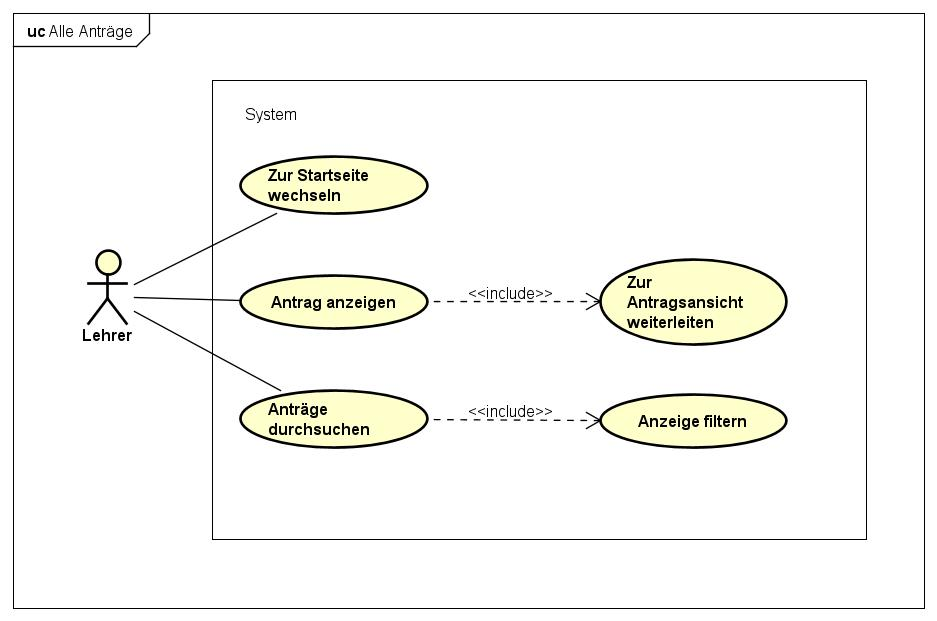
\includegraphics[width=1\linewidth]{images/uc-all}
	\caption[Use Case Diagramm Alle Anträge]{Das Use Case Diagramm für die \enquote{Alle Anträge} Seite}
	\label{fig:ucAll}
\end{figure}
\newpage
\paragraph{Ansicht Aktive Anträge}
~\\
Auf der \enquote{Aktive Anträge} Seite, sieht man alle Anträge, die aktiv sind (also in Bearbeitung oder vorerst abgelehnt) und mit denen man in Verbindung steht. Diese können über das Menü auf der rechten Seite geöffnet werden (Abbildung 6.10).
\begin{figure}[H]
	\centering
	\includegraphics[width=1\linewidth]{images/Mockup-Aktive-Anträge}
	\caption[Mokup aktive Anträge]{Das Mockup, welches alle aktiven Anträge einer gewissen Person veranschaulicht}
	\label{fig:mockupAktive}
\end{figure}
Zur Veranschaulichung der oben genannten Prozesse ist in Abbildung 6.11 ein beispielhaftes Use-Case Diagramm zu sehen: 
\begin{figure}[H]
	\centering
	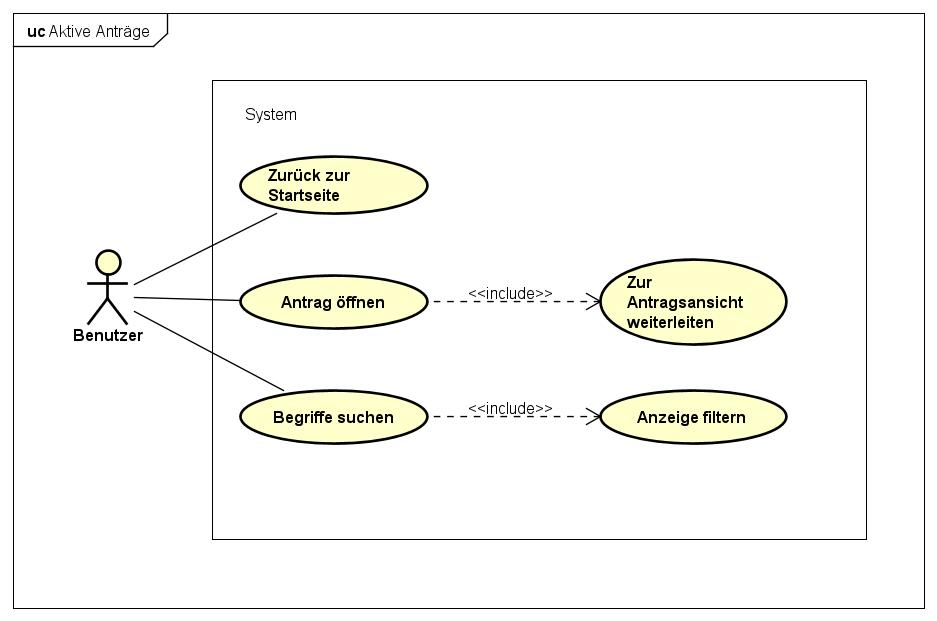
\includegraphics[width=1\linewidth]{images/uc-active}
	\caption[Use Case Diagramm Aktive Anträge]{Das Use Case Diagramm für die \enquote{Aktive Anträge} Seite}
	\label{fig:ucAktiv}
\end{figure}
\newpage
\paragraph{Administrator Ansicht}
~\\
Auf der Administrator Seite können bestimmte Nutzer (wie AV, Rechnungsstelle, etc.) Anträge verwalten. Wie man auf der Abbildung 6.12 sehen kann werden dem Benutzer einige wichtige Daten in einer durchsuchbaren und filtrierbaren Tabelle angezeigt. Um den Antrag anzunehmen oder abzulehnen kann der \enquote{Öffnen} Knopf auf der rechten Seite der Tabelle betätigt werden.
\begin{figure}[H]
	\centering
	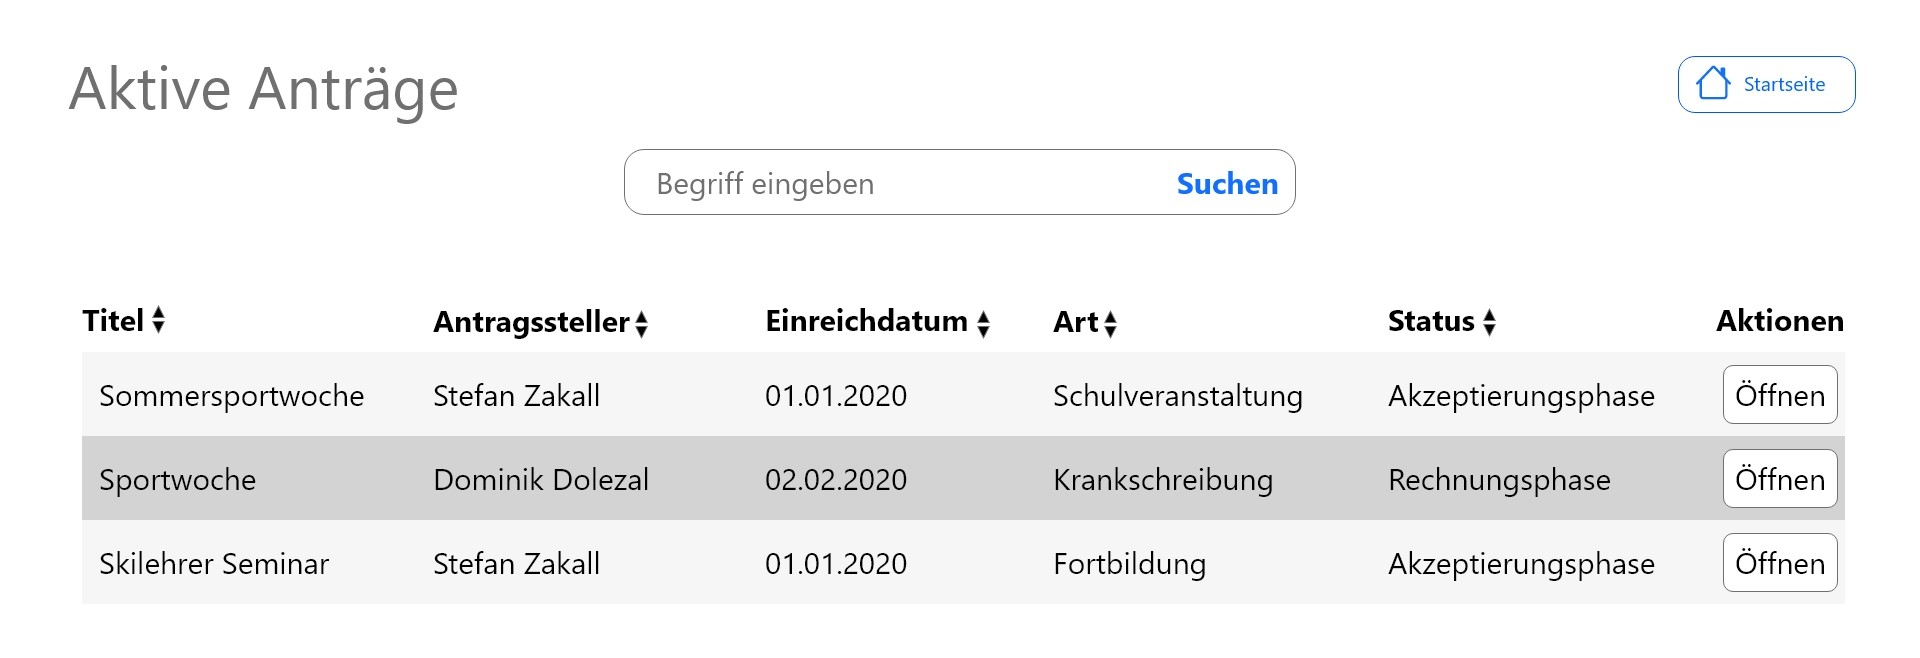
\includegraphics[width=1\linewidth]{images/Mockup-Admin}
	\caption[Mockup Adminansicht]{Das Mockup, der Admin Ansicht, zum akzeptieren und ablehnen von Anträgen}
	\label{fig:mockupAdmin}
\end{figure}
Zur Veranschaulichung der oben genannten Prozesse ist in Abbildung 6.13 ein beispielhaftes Use-Case Diagramm zu sehen: 
\begin{figure}[H]
	\centering
	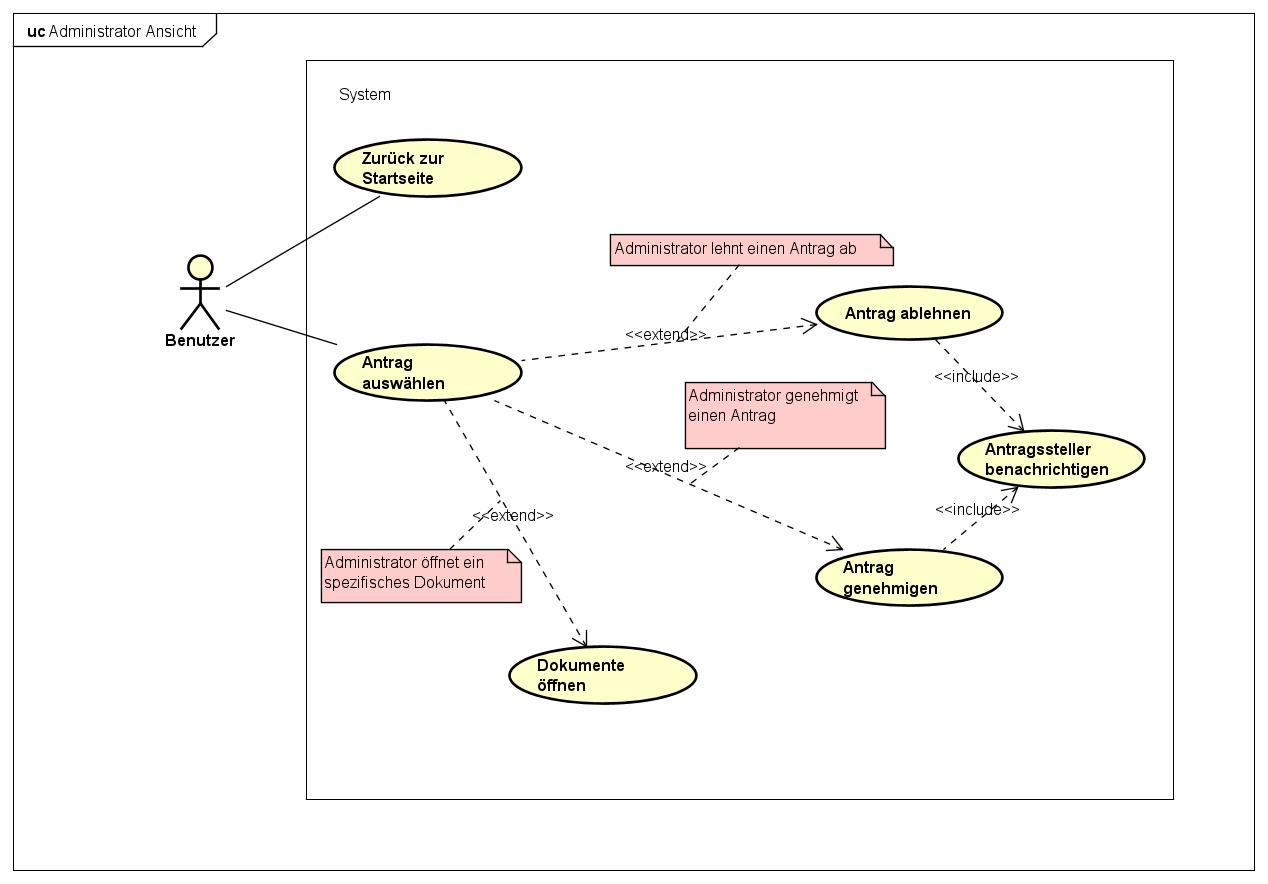
\includegraphics[width=1\linewidth]{images/uc-admin}
	\caption[Use Case Diagramm Adminansicht]{Das Use Case Diagramm für die Administrator Ansicht}
	\label{fig:ucAdmin}
\end{figure}
\paragraph{Antragsansicht}
~\\
Hat der Nutzer einen bestimmten Antrag oder eine Neuigkeit zu einem Antrag ausgewählt, wird er auf die passende Antragsseite weitergeleitet (Abbildung 6.14). Auf dieser Seite ist es möglich vorhandene Daten zu bearbeiten. Außerdem kann der Nutzer PDF-Dateien zu allen vorhandenen Anträgen generieren.
\begin{figure}[H]
	\centering
	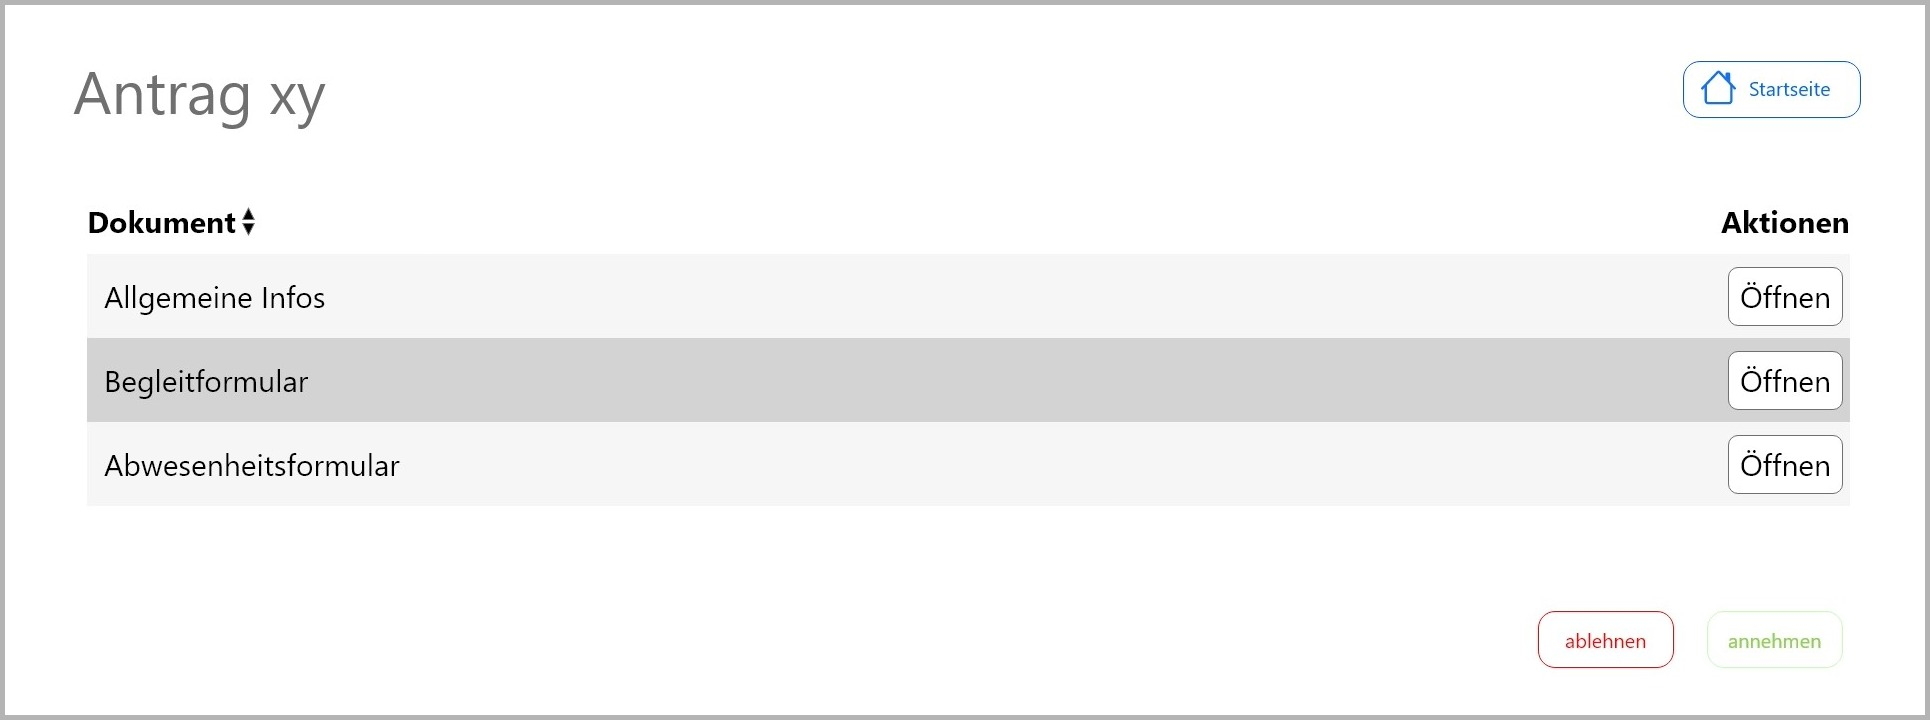
\includegraphics[width=1\linewidth]{images/Mockup-Antragsansicht}
	\caption[Mockup Antragsansicht]{Das Mockup, welches einen eingereichten Antrag veranschaulicht}
	\label{fig:mockupAntrag}
\end{figure}
Zur Veranschaulichung der oben genannten Prozesse ist in Abbildung 6.15 ein beispielhaftes Use-Case Diagramm zu sehen: 
\begin{figure}[H]
	\centering
	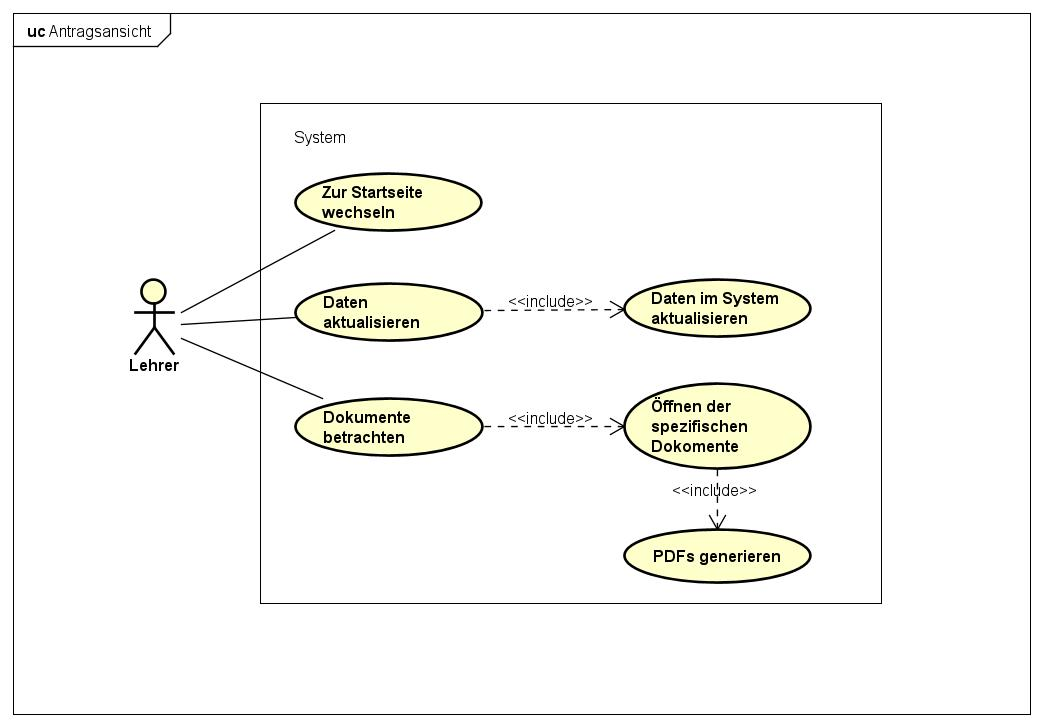
\includegraphics[width=1\linewidth]{images/uc-antrag}
	\caption[Use Case Diagramm Antragsansicht]{Das Use Case Diagramm für die Antragsansicht}
	\label{fig:ucAntrag}
\end{figure}